\documentclass{beamer}
\usetheme{Singapore}
\usepackage{changepage}

%\usepackage{pstricks,pst-node,pst-tree}
\usepackage{amssymb,latexsym}
\usepackage{tikz}
\usepackage{graphicx}
\usepackage{fancyvrb}
\usepackage{hyperref}
\usepackage{fancybox}
\usepackage[listings]{tcolorbox}

\definecolor{codegreen}{rgb}{0,0.6,0}
\definecolor{codegray}{rgb}{0.5,0.5,0.5}
\definecolor{codepurple}{rgb}{0.58,0,0.82}
\definecolor{backcolour}{rgb}{0.95,0.95,0.92}

\lstdefinestyle{mystyle}{
    language=Python,
    backgroundcolor=\color{backcolour},   
    commentstyle=\color{codegreen},
    keywordstyle=\color{magenta},
    numberstyle=\tiny\color{codegray},
    stringstyle=\color{codepurple},
    basicstyle=\ttfamily\footnotesize,
    breakatwhitespace=false,         
    breaklines=true,                 
    captionpos=b,                    
    keepspaces=true,                 
    numbers=left,                    
    numbersep=5pt,                  
    showspaces=false,                
    showstringspaces=false,
    showtabs=false,                  
    tabsize=2,
    escapechar=|,
    frame=single
}

\lstset{style=mystyle}


\newcommand{\bi}{\begin{itemize}}
\newcommand{\li}{\item}
\newcommand{\ei}{\end{itemize}}
\newcommand{\Show}[1]{
\begin{center}
\shadowbox{\begin{minipage}{0.8\textwidth}
          #1
          \end{minipage}}
\end{center}
}
\newcommand{\arrow}{\ensuremath{\rightarrow}}

\newcommand{\uparr}{\ensuremath{\uparrow}}


\newcommand{\fig}[2]{\centerline{\includegraphics[width=#1\textwidth]{#2}}}

\newcommand{\bfr}[1]{\begin{frame}[fragile]\frametitle{{ #1 }}}
\newcommand{\efr}{\end{frame}}

\newcommand{\cola}{\begin{columns}\begin{column}{0.5\textwidth}}
\newcommand{\colb}{\end{column}\begin{column}{0.5\textwidth}}
\newcommand{\colc}{\end{column}\end{columns}}


\title{Think Python 2e, Chapter 7 Notes}
\author{Geoffrey Matthews}

\begin{document}

\begin{frame}
\maketitle

\end{frame}

\bfr{Reassignment}
\cola
\begin{lstlisting}
>>> x = 5
>>> x
5
>>> x = 7
>>> x
7
\end{lstlisting}
\colb
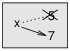
\includegraphics{thinkpython2008}

\bigskip 

State diagram
\colc

\end{frame}

\bfr{Updating variables}
\begin{lstlisting}
>>> x = x + 1
NameError: name 'x' is not defined
\end{lstlisting}

Must be initialized first:

\begin{lstlisting}
>>> x = 0
>>> x = x + 1
\end{lstlisting}

\end{frame}

\bfr{The {\tt while} statement}

\cola
\begin{lstlisting}
def countdown(n):
    while n > 0:
        print(n)
        n = n - 1
    print('Blastoff!')
\end{lstlisting}
\pause
\colb
\begin{lstlisting}
def countdown(n):
    if n > 0:
        print(n)
        n = n - 1
    print('Blastoff!')
\end{lstlisting}
\colc

\end{frame}

\bfr{The Collatz Sequence}
\begin{lstlisting}
def sequence(n):
    print('Collatz: ', end='')
    while n != 1:
        print(n, end=', ')
        if n % 2 == 0:        # n is even
            n = n // 2
        else:                 # n is odd
            n = n*3 + 1
    print(n)
\end{lstlisting}
\begin{lstlisting}
Collatz: 3, 10, 5, 16, 8, 4, 2, 1
Collatz: 512, 256, 128, 64, 32, 16, 8, 4, 2, 1
Collatz: 513, 1540, 770, 385, 1156, 578, 289, 868, 434, 217, 652, 326, 163, 490, 245, 736, 368, 184, 92, 46, 23, 70, 35, 106, 53, 160, 80, 40, 20, 10, 5, 16, 8, 4, 2, 1
\end{lstlisting}

\end{frame}

\bfr{break}
\begin{lstlisting}
while True:
    line = input('> ')
    if line == 'done':
        break
    print(line)

print('Done!')
\end{lstlisting}

\end{frame}
\bfr{Newton's Method}
Find the square root of a number by iteration.

\[
\begin{array}{cccccc}
n & x & x^2 & n/x & \frac{x + n/x}{2} & \left(\frac{x + n/x}{2}\right)^2 \\
5 & 10 & 100 & 0.5 & 5.25 & 27.56\\
5 & 5.25 & 27.56 & 0.95 & 3.1 & 9.62\\
5 & 3.1 & 9.62 & 1.61 & 2.36 & 5.55\\
5 & 2.36 & 5.55 & 2.12 & 2.24 & 5.01\\
5 & 2.24 & 5.01 & 2.23 & 2.24 & 5.0\\
\end{array}
\]
Final answer:
\[
2.23607010853285^2 = 5.000009530274112
\]
\end{frame}
\bfr{Newton's Method}
\[
\begin{array}{cccccc}
n & x & x^2 & n/x & \frac{x + n/x}{2} & \left(\frac{x + n/x}{2}\right)^2 \\
5000 & 10 & 100 & 500.0 & 255.0 & 65025.0\\
5000 & 255.0 & 65025.0 & 19.61 & 137.3 & 18852.37\\
5000 & 137.3 & 18852.37 & 36.42 & 86.86 & 7544.62\\
5000 & 86.86 & 7544.62 & 57.56 & 72.21 & 5214.56\\
5000 & 72.21 & 5214.56 & 69.24 & 70.73 & 5002.21\\
\end{array}
\]
Final answer:
\[
70.72628275743688^2 = 5002.207072684913
\]

\end{frame}

\bfr{Newton's Method}
\begin{lstlisting}
def newton(n):
    x = 10
    while abs(x**2/n - 1) > 1e-5:
        x = (x + n/x)/2
    return x
\end{lstlisting}

\end{frame}
\bfr{Algorithms}
\bi
\li Newton's method is an {\bf algorithm} for finding square roots.
\li An algorithm is a method for solving a class of problems.
\li There are other ways of finding square roots, using different
algorithms.
\bi \li long division \li binary search \ei
\li Which algorithm is best for which problem is real computer science.
\ei

\end{frame}

\bfr{Debugging by bisection}
\bi
\li Divide the program roughly in half.
\li Find an intermediate result there.
\li Test to see if this result is correct.
\bi
\li If no, the problem is in the first half
\li If yes, the problem is in the second half
\ei
\li Now divide the subset of the program in half, and repeat.
\ei
\end{frame}

\bfr{Vocabulary}
\begin{description}
\li[reassignment:]
Assigning a new value to a variable that already exists.
\li[update:]
An assignment where the new value of the variable depends on the old.
\li[initialization:]
An assignment that gives an initial value to a variable that will be updated.
\li[increment:]
An update that increases the value of a variable (often by one).
\li[decrement:]
An update that decreases the value of a variable.
\li[iteration:]
Repeated execution of a set of statements using either a recursive function call or a loop.
\li[infinite loop:]
A loop in which the terminating condition is never satisfied.
\li[algorithm:]
A general process for solving a category of problems.
\end{description}
\end{frame}

\end{document}
